\section{Machine Learning Applications for HMM}
\label{sec:ml}

% introducere in invatare automata + categorisire probleme
\subsection{Machine Learning}
\label{sec:hmm_in_ml}

\begin{frame}
  \frametitle{What is Machine Learning?}
  \begin{block}{Machine Learning}
    ..\alert{Trascau} is a beautiful horse.
  \end{block}
\end{frame}

\begin{frame}
  \frametitle{Machine Learning Applications}
  \begin{itemize}
  \item Computer Vision: Google Car
  \item Machine Translation
  \item Speech Recognition
  \item Recommender Systems
  \item Intelligent Advertising
  \end{itemize}
\end{frame}

% aplicatii specifice hmm-urilor
% de ce am ales hmm-urile 
\subsection{Where do HMMs fit into Machine Learning?}
\label{sec:apps}

\begin{frame}
  \frametitle{Machine Learning Classification}
  Types of Machine Learning Problems
  \begin{itemize}
  \item Regression
  \item Classification
  \item Reinforcement Learning
  \end{itemize}
  \begin{itemize}
  \item supervised learning (eg. ..)
  \item unsupervised
  \end{itemize}
\end{frame}

%% aici facem tranzitie de la problema generala de ML
%% la probleme cu secvente temporale, markov stuff, dbn shit
%% adica HMM-uri :))

%% Markov models, Dynamic Bayesian Networks
\begin{frame}
  \frametitle{Sequence / Temporal problems (I)}
  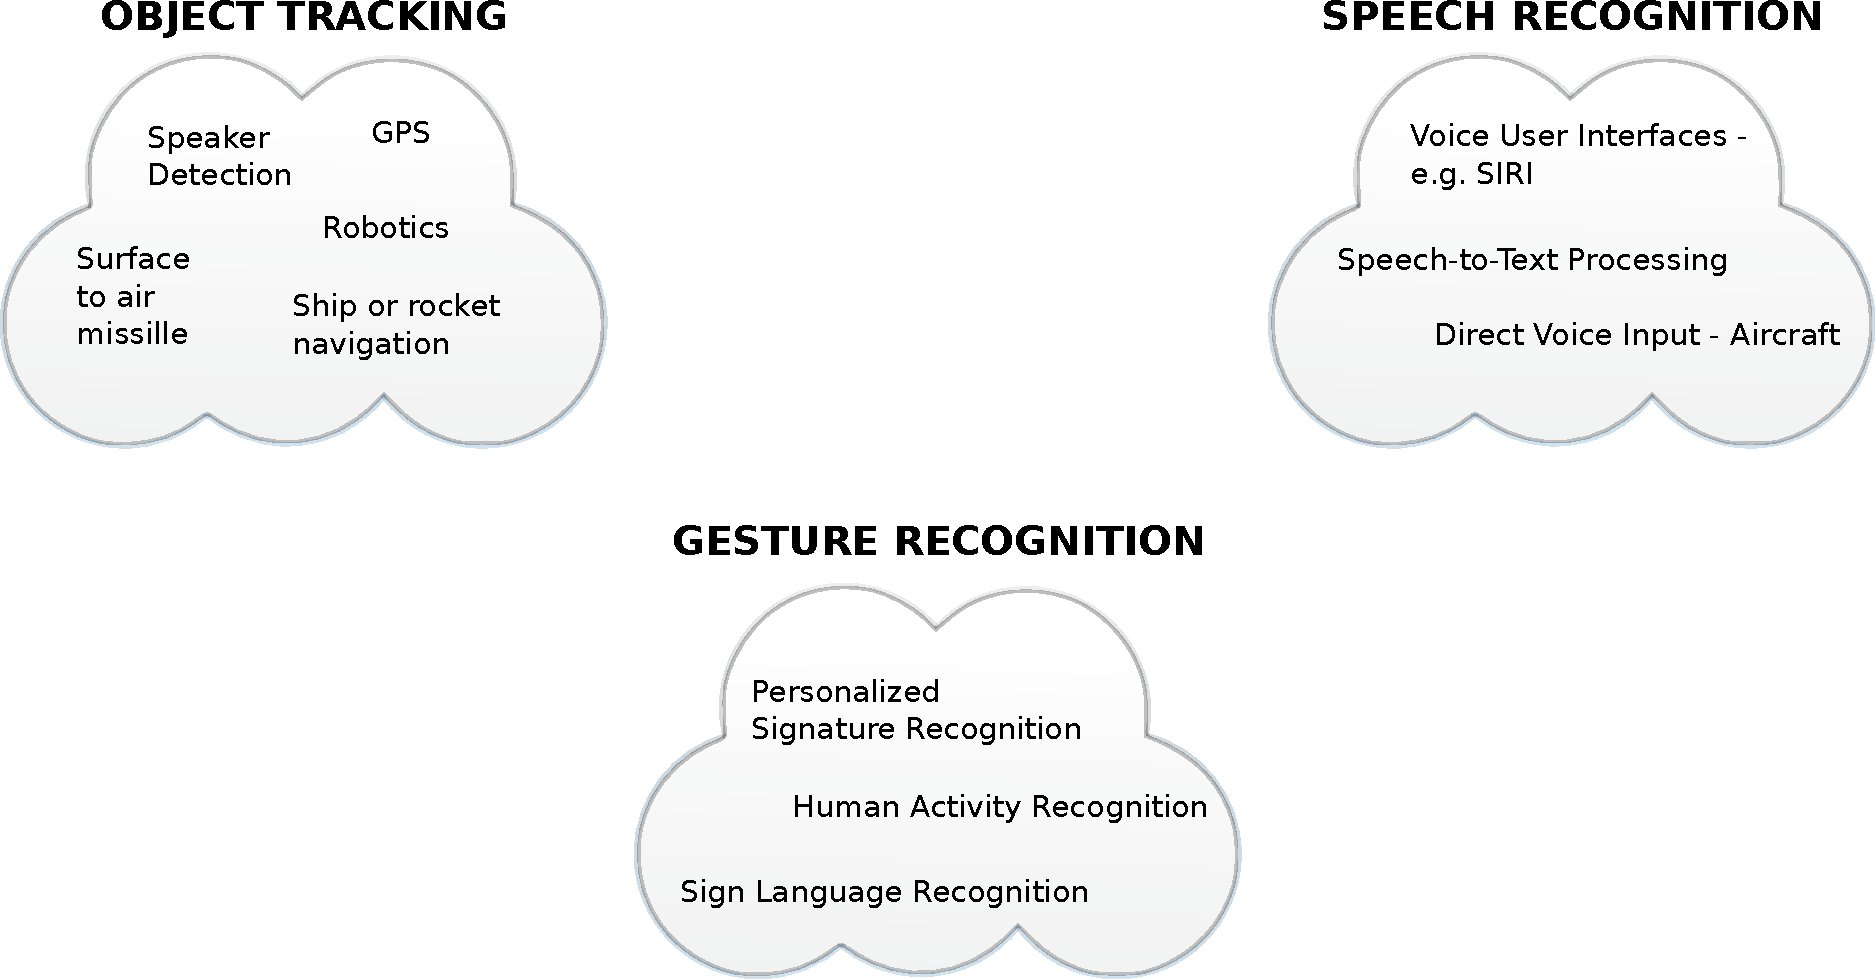
\includegraphics[width=\textwidth]{images/time_series_problems_1.pdf}
\end{frame}

\begin{frame}
  \frametitle{Sequence / Temporal problems (II)}
  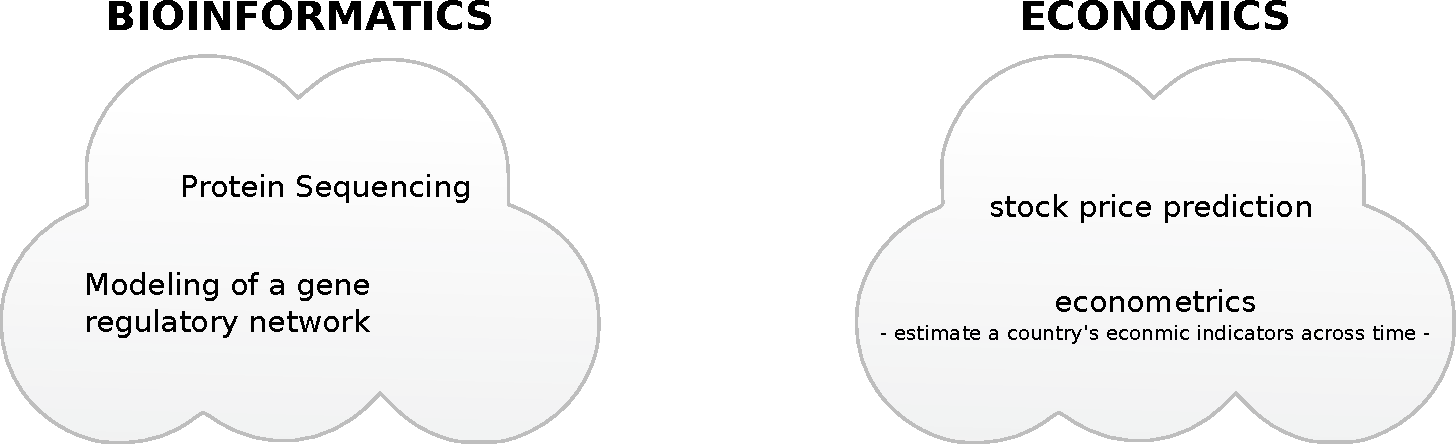
\includegraphics[width=\textwidth]{images/time_series_problems_2.pdf}
  %Koller and Frideman au scris in \cite{KollerFriedman09}
  % temporal sequences
  % DBN for ts
  % HMM as a special case of DBN
\end{frame}

\begin{frame}
  \frametitle{Sequence / Temporal problems (III)}
  Some tools of the trade:
  
  \begin{itemize}
  	\item DBN
  	\item Kalman Filters
  	\item HMMs
  \end{itemize}
  %Koller and Frideman au scris in \cite{KollerFriedman09}
  % temporal sequences
  % DBN for ts
  % HMM as a special case of DBN
\end{frame}


% descrierea a ceea ce inseamna Probabilistic Reasoning over Time (capitol 15.2 AI a modern approach)
% 	- states and observations
%	- stationary process, Markov assumption, Sensor model
%	- inference in temporal models
%		- filtering
%		- prediction
%		- smoothing (hindsight)
%		- most likely explanation
%		- model learning
\begin{frame}
  \frametitle{Probabilistic Reasoning over Time}
  %% poza cu trei stari
  
  %% formule :)
  
\end{frame}

%% exemplu de hmm, fura alex exemplul cu sad si happy

%% Aplicatii ale HMM-urilor
%% TODO
\begin{frame}
  \frametitle{Applications for HMMs}
  \begin{itemize}[<+->]
  \item Robot localization
  \item DNA sequence analysis
  \item Hand-Writing Recognition
  \item Speech Recognition (newxt on baywatch)
  \end{itemize}
\end{frame}
